\section{Исследовательская часть}

\subsection{Цель исследования}

Целью исследования является оценка производительности разработанного алгоритма программной растеризации. Необходимо установить зависимость среднего времени отрисовки одного кадра от количества геометрических объектов (шестеренок) в сцене.

\subsection{Технические характеристики}

Исследование проводилось на ноутбуке со следующими характеристиками:
\begin{itemize}
	\item операционная система --- Debian Unstable GNU/Linux с ядром версии 6.17.12;
	\item процессор --- AMD Ryzen 5 7535HS с 6 физическими ядрами и 12 логическими ядрами с максимальной тактовой частотой 4.60~ГГц~\cite{ryzen};
	\item оперативная память --- 16~Гбайт типа LPDDR5 в 4 каналах с тактовой частотой 6400~MГц.
\end{itemize}

\subsection{Алгоритм проведения исследования}

\begin{enumerate}
	\item Приложение запускается в режиме тестирования производительности.
	\item Камера фиксируется.
	\item Производится замер времени выполнения функции отрисовки кадра для количества шестеренок на сцене от 2 до 100 с шагом 2.
	\item Для каждого замера производится 100 повторений (отрисовок кадра), усредняется и сохраняется в файл.
\end{enumerate}

\subsection{Результаты исследования}

В таблице \ref{table:benchmark} приведены полученные данные.

\begin{table}[H]
	\caption{Зависимость времени рендеринга от количества объектов}
	\label{table:benchmark}
	\normalsize
	\begin{tabular}{|c|c||c|c||c|c|}
		\hline
		N, шт. & T, мс   & N, шт. & T, мс   & N, шт. & T, мс   \\ \hline
		2      & 21.3832 & 36     & 32.0729 & 70     & 44.1520 \\ \hline
		4      & 22.2666 & 38     & 32.5122 & 72     & 44.5449 \\ \hline
		6      & 22.9500 & 40     & 33.4331 & 74     & 45.1821 \\ \hline
		8      & 23.7334 & 42     & 34.4030 & 76     & 45.7830 \\ \hline
		10     & 24.3168 & 44     & 35.3910 & 78     & 45.9031 \\ \hline
		12     & 25.4002 & 46     & 35.7086 & 80     & 46.9414 \\ \hline
		14     & 25.4836 & 48     & 36.0991 & 82     & 47.0862 \\ \hline
		16     & 26.3670 & 50     & 36.8994 & 84     & 47.7650 \\ \hline
		18     & 27.0504 & 52     & 37.7999 & 86     & 48.1849 \\ \hline
		20     & 27.5338 & 54     & 37.6583 & 88     & 48.7174 \\ \hline
		22     & 28.0172 & 56     & 38.1220 & 90     & 49.0622 \\ \hline
		24     & 29.1006 & 58     & 38.9347 & 92     & 50.0099 \\ \hline
		26     & 29.3729 & 60     & 39.4367 & 94     & 51.2052 \\ \hline
		28     & 30.0054 & 62     & 40.4037 & 96     & 52.6742 \\ \hline
		30     & 30.2218 & 64     & 41.5348 & 98     & 53.9166 \\ \hline
		32     & 30.6255 & 66     & 42.3975 & 100    & 54.8800 \\ \hline
		34     & 31.1867 & 68     & 43.3006 &        &         \\ \hline
	\end{tabular}
\end{table}

На рисунке \ref{img:graph} представлен график зависимости времени кадра от количества шестеренок.

\begin{figure}[H]
	\centering
	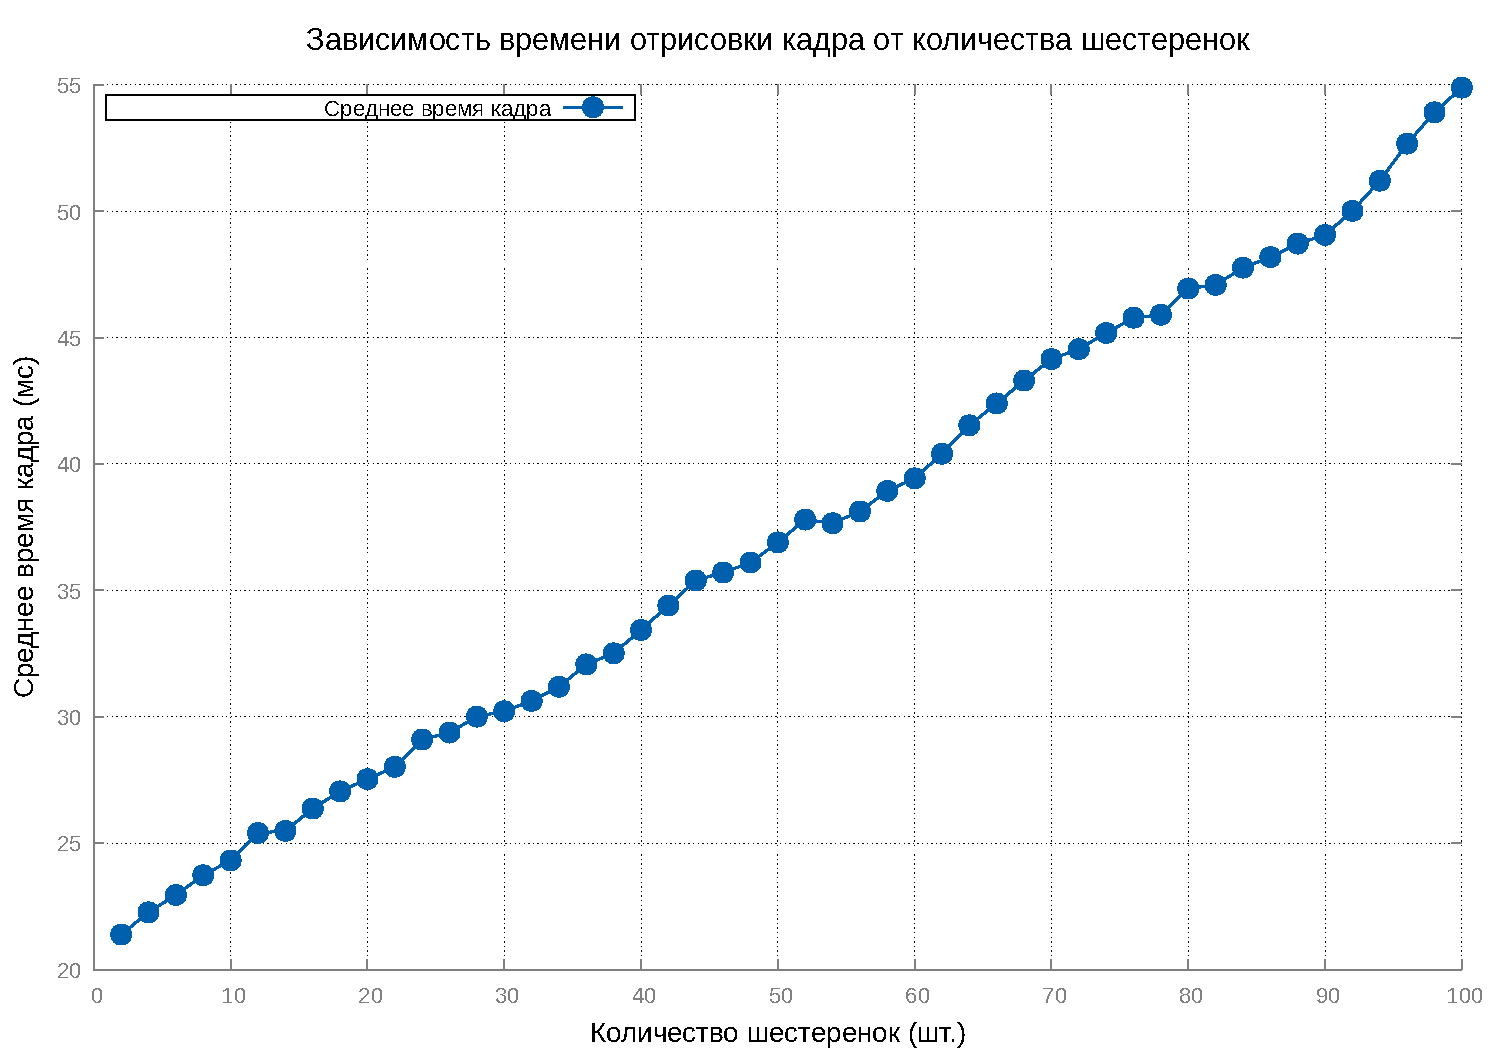
\includegraphics[width=0.9\textwidth]{img/benchmark_graph.pdf}
	\caption{График зависимости времени рендеринга от числа объектов}
	\label{img:graph}
\end{figure}

\subsection{Анализ результатов}

Зависимость времени рендеринга от количества объектов носит линейный характер. Это согласуется с теоретической оценкой сложности алгоритма растеризации и Z-буфера.

При увеличении количества объектов с 2 до 100 (рост в 50 раз), время кадра увеличилось с $\approx 21$ мс до $\approx 55$ мс (рост в 2.6 раза). Это свидетельствует о том, что значительную часть времени занимает отрисовка статического окружения и очистка буферов высокого разрешения, а добавление новой геометрии обрабатывается достаточно эффективно.

При 100 шестеренках время кадра составляет 54.8 мс, что соответствует частоте кадров $\approx 18$ FPS, что обеспечивает достаточную интерактивность приложения.

\subsection*{Вывод}

Проведенное исследование подтвердило линейную зависимость времени рендеринга от количества геометрических примитивов в сцене. Установлено, что разработанная программная реализация обеспечивает приемлемую производительность при нагрузке в 100 сложных объектов с учетом затрат на расчет теней и освещения на центральном процессоре. Полученные характеристики подтверждают эффективность выбранных алгоритмов и структур данных.
